\subsection{ダイオード}
半導体内部には,電子と正孔がキャリアとして存在している。
真性半導体には4価のシリコンがよく使われる。
真性半導体に微量の不純物を混入させたものを不純物半導体と言い,不純物としてリンやヒ素のような5価の元素(ドナー)を用いたものをn型半導体,ホウ素やガリウムのような3価の元素(アクセプタ)を用いたものをp型半導体と呼ぶ。

\wfig{fig1}のように,p型半導体とn型半導体を接合し,端子を付けたものをダイオードと呼ぶ。
ダイオード内部において,正孔はp型半導体内では多数キャリア,n型半導体内では少数キャリアであるから,より密度の大きいp型領域からn型領域へ流れ込む。
この現象を拡散と呼ぶ。
また,n領域へ拡散した正孔はn領域内の電子と結合し,双方とも消滅する。
したがって,n領域では正に帯電したドナーイオンが,p領域では負に帯電したアクセプタイオンのみが残り,平衡状態となる。
この結果,pn接合近傍にはキャリアの存在しない空乏層が形成される。
空乏層では,電化分布によりp領域側からn領域側へ電位差が発生し,これを拡散電位と呼ぶ。

\begin{figure}[!h]
 \centering
 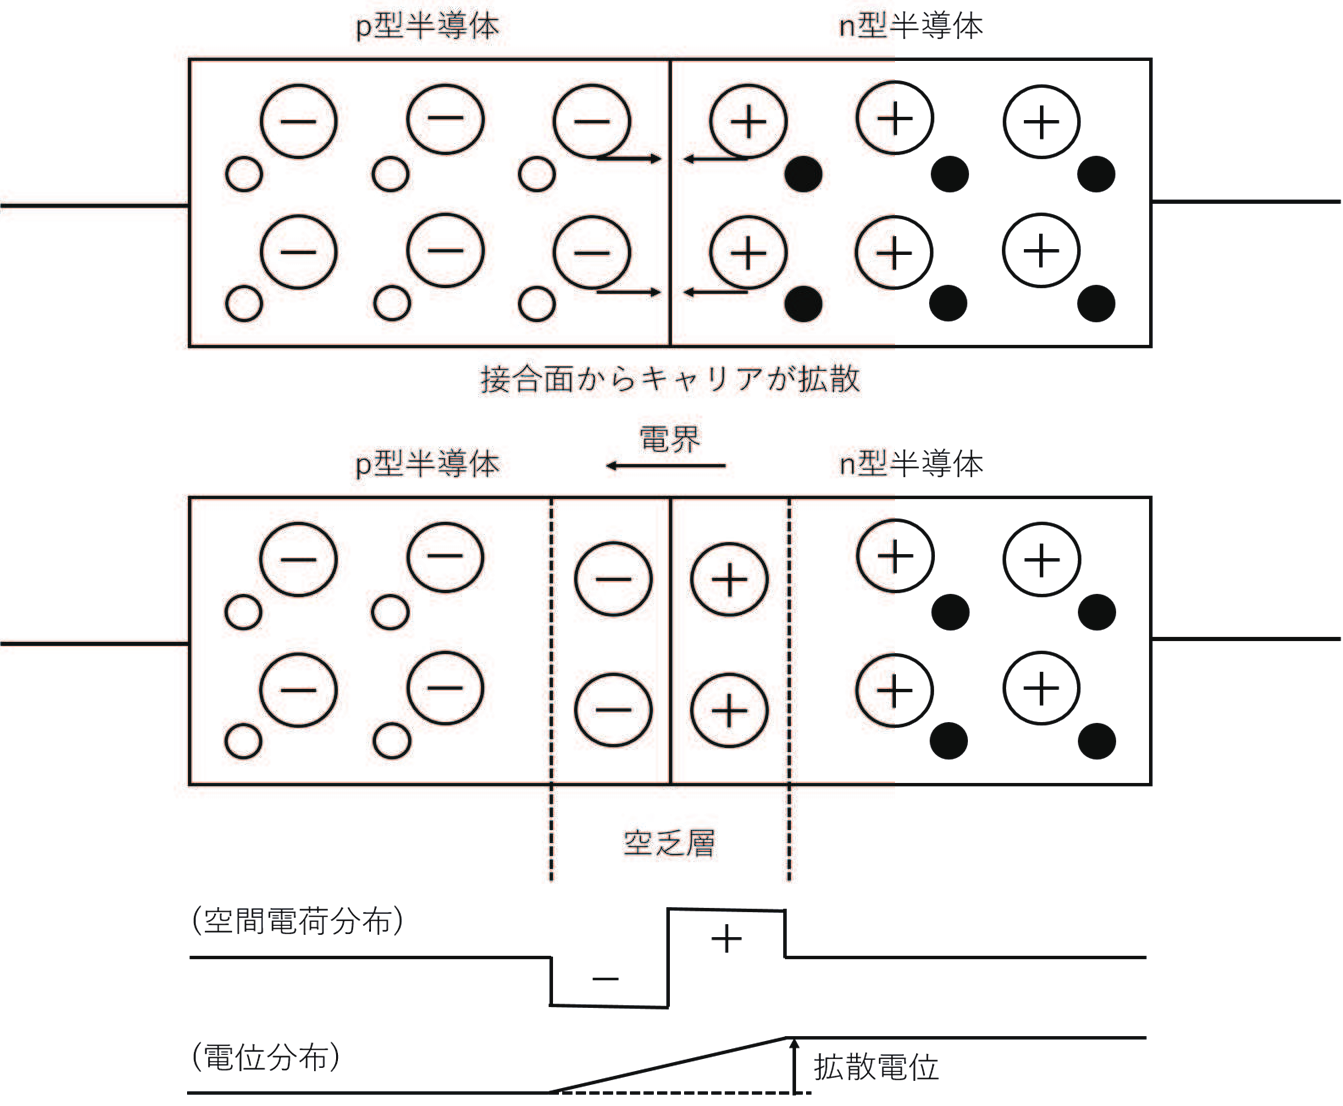
\includegraphics[width=8.2cm]{./pdfs/fig1.pdf}
 \caption{pn接合と空乏層}
 \label{fig:fig1}
\end{figure}%

\wfig{fig2}のようにp型半導体に正,n型半導体に負の電圧を加えると,p領域とn領域の電位差は拡散電圧+印加電圧となり,電圧差が減少するため拡散電位により阻止されていたキャリアの拡散が起こる。
このとき,ダイオードに印加した電圧,流れた電流を,それぞれ順方向電圧,順方向電流という。
逆に,n型半導体に正,p型半導体に負の電圧を加えると,p領域とn領域の電圧差が大きくなるため電流は殆ど流れなくなる。
このとき,ダイオードに加えた電圧,流れた電流を,それぞれ逆方向電圧,逆方向電流という。
また,この電圧のかけ方を逆バイアスという。

\begin{figure}[!t]
 \centering
 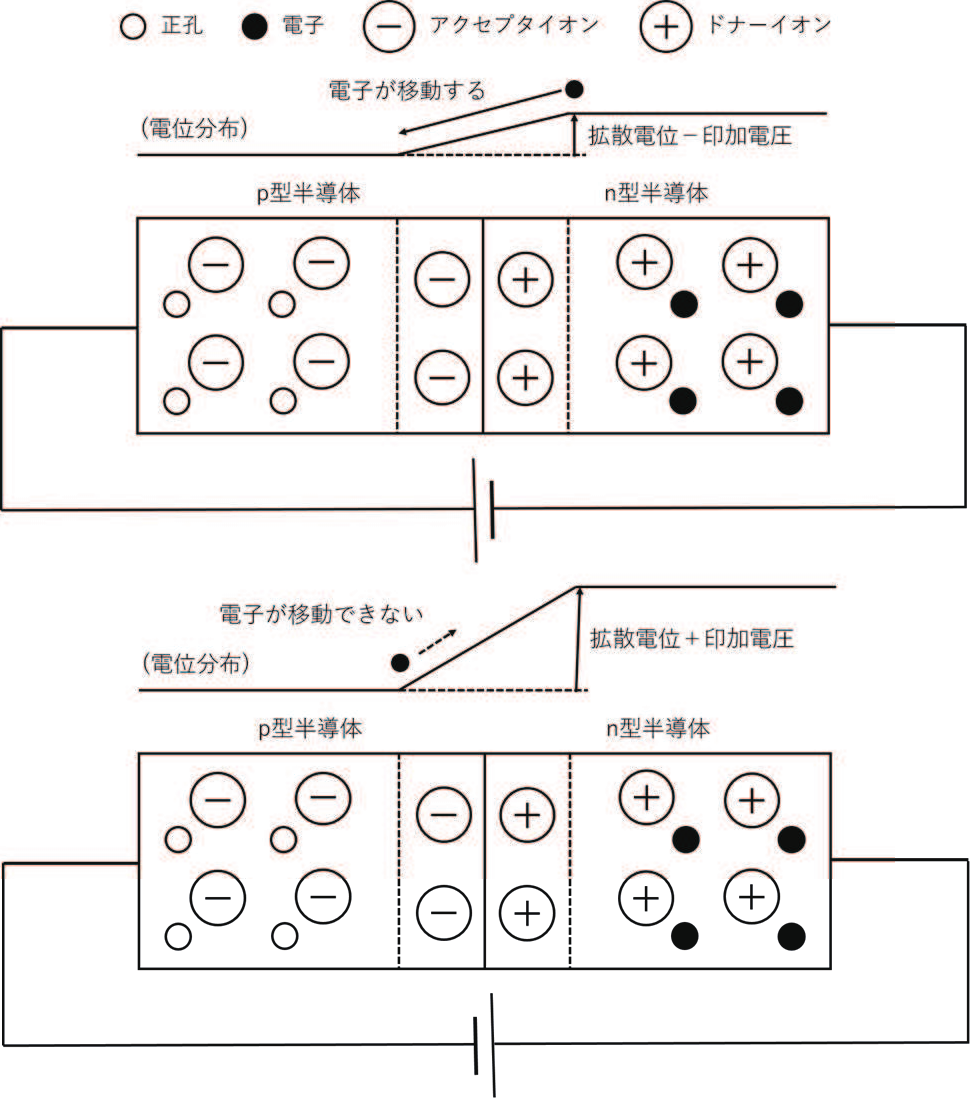
\includegraphics[height=8.0cm]{./pdfs/fig2.pdf}
 \caption{ダイオードの動作原理}
 \label{fig:fig2}
\end{figure}%

\subsection{ツェナーダイオード}
ツェナーダイオードは定電圧ダイオードとも呼ばれ,加わる電圧がある一定の値(ツェナー電圧)を上回ると,急激に電流が流れるようになる素子である。
このとき流れる電流をツェナー電流と呼ぶ。
入力電圧の増加に伴いツェナー電流が増加するため,出力電圧は一定に保たれる。
すなわち,ツェナーダイオードは端子間電圧がツェナー電圧以上ならON,ツェナー電圧以下ならOFFといったようにスイッチと似たような動作をして,ほぼ一定の電圧を維持する素子である。

\subsection{太陽電池}
太陽電池は様々な種類のものがあるが,本実験では最も基本的な構造である結晶シリコン太陽電池を用いる。
結晶シリコン太陽電池の構造は,\wfig{fig3}のような上段がn 形半導体,下段がp 形半導体となっており,pn結合している。
\wfig{fig4}で示すように,光が照射されると光のエネルギーにより接合面の電子はn形半導体へ,正孔はp形半導体へ移動し,起電力が発生する(光起電力効果)。
この起電力は,光が照射されている間は持続し外部に負荷を接続しておけば電力を供給することができる。
また,電子は負荷を通ってp形半導体に戻り,正孔と結合する。
\begin{figure}[htb]
	\centering
	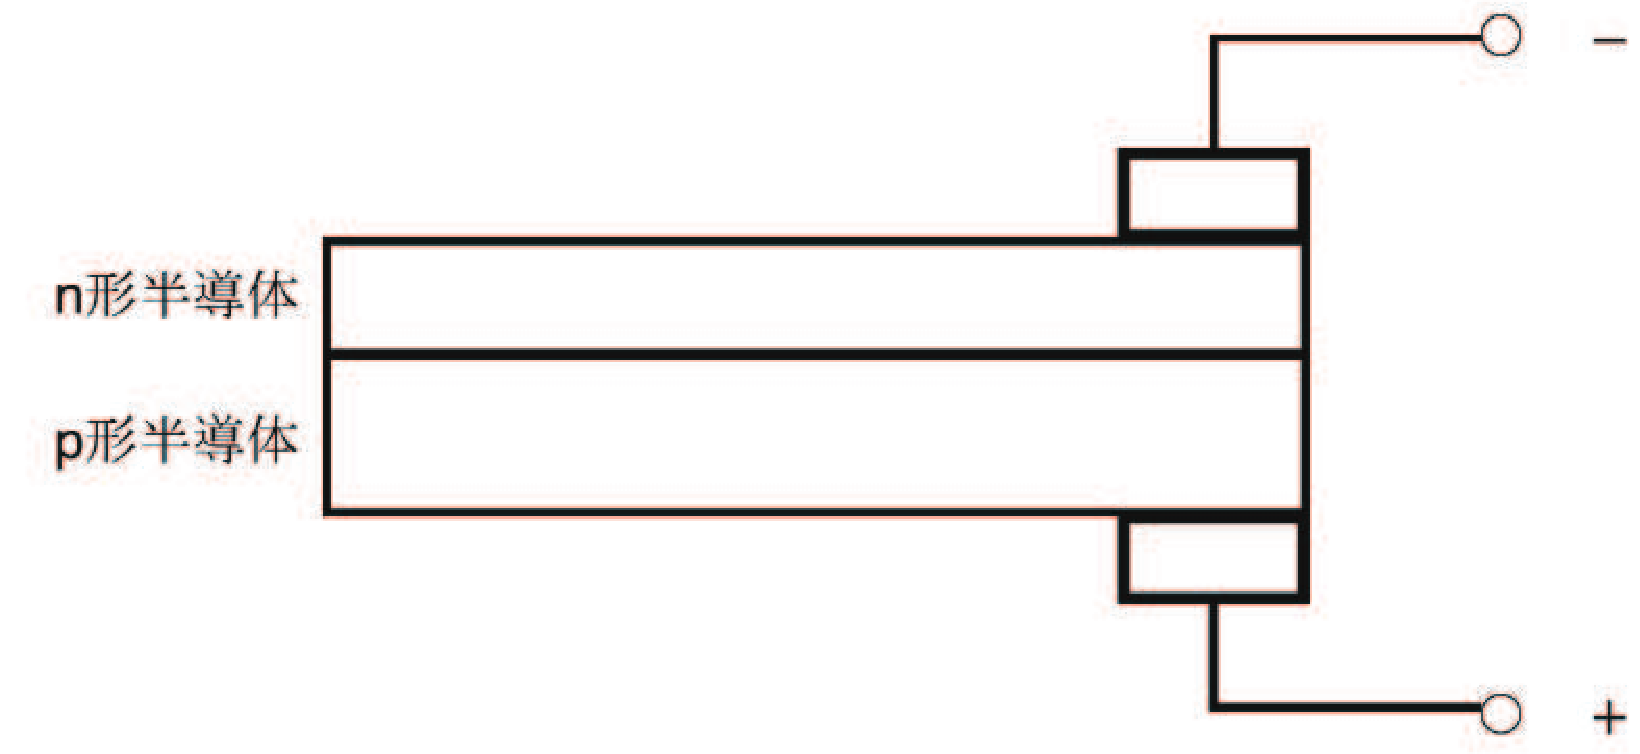
\includegraphics[width=6.3cm]{./pdfs/fig3.pdf}
	\caption{結晶シリコン太陽電池の構造}
	\label{fig:fig3}
\end{figure}

\begin{figure}[htb]
	\centering
	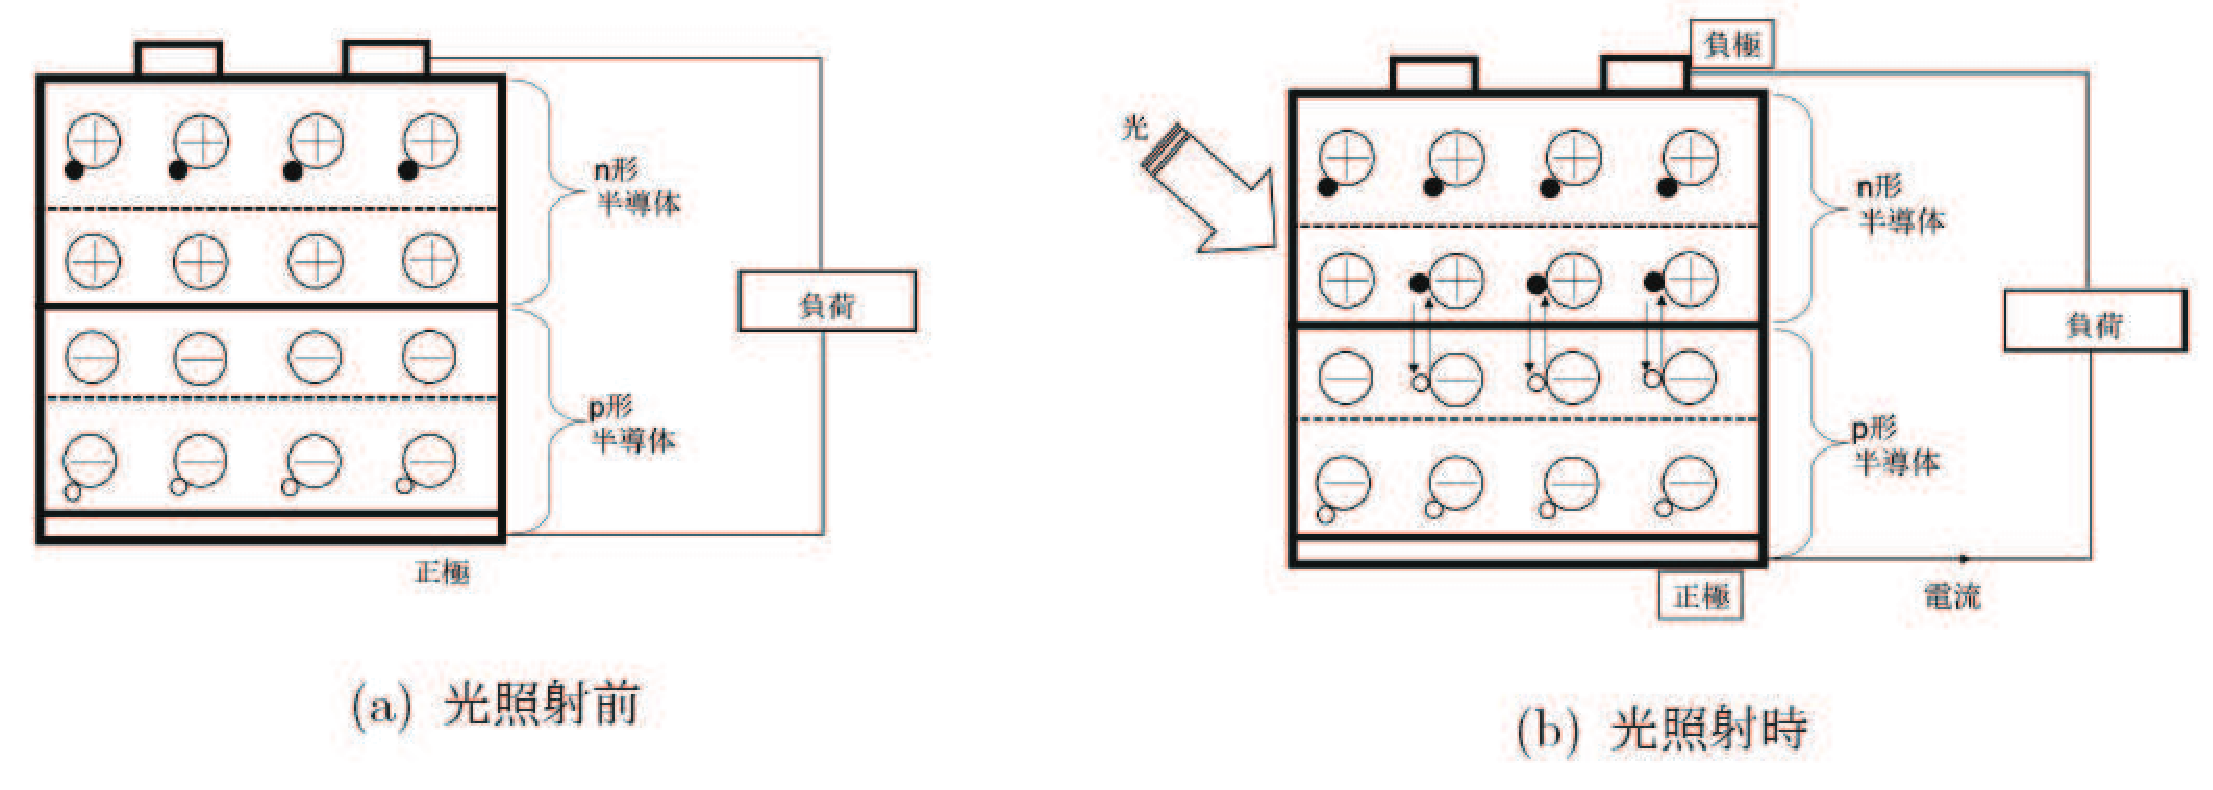
\includegraphics[width=12cm]{./pdfs/fig4.pdf}
	\caption{太陽電池の動作原理}
	\label{fig:fig4}
\end{figure}

太陽電池の電流--電圧特性は\wfig{fig5}に示したようなダイオードの特性を下にシフトした特性となる。
ここで電流値は負の値になるが,正に消費と考えていたので負の値は発電していることを意味する。
一般的には,発電した電力も正の値で表現するので,縦軸を反転させる(\wfig{fig5}参照)。
また,太陽電池の電流--電圧特性をI-Vカーブ,電力--電圧特性をP-Vカーブと呼ぶ。
\wfig{fig6}に示すように,I-V カーブは第1象限のみを表示する。


ここで電圧が0\,Vになる(短絡する》 時の電流を短絡電流($I_{\mathrm{sc}}$),電流が0\,A になる電圧を解放電圧($V_{\mathrm{oc}}$)と呼ぶ。
また,縦軸を電力とした\wfig{fig6}に示すP-Vカーブからわかる通り,太陽電池はどのようなどのような電圧で利用しても同じ電力を得られるわけではない。
太陽電池を有効に活用するためには,発電電力が最大になる最大電力点で利用する必要がある。

ここで,発電電力が最大になる電力を最大電力($P_{\mathrm{max}}$),その時の電圧を最適動作電圧($V_{\mathrm{pm}}$) と呼ぶ。
$P_{\mathrm{max}}$は,気象条件によって大きく変化し$V_{\mathrm{pm}}$も変化してしまう。
そのため,太陽電池を利用したシステム(太陽光発電システム)では,常に$P_{\mathrm{max}}$ を追従する制御であるMPPT制御(Maximum Power Point Tracking:最大電力点追尾)が具備されている。
MPPTには様々な手法があるが,その手法を考える上でも太陽電池のI-Vカーブの測定は非常に重要である。

\begin{figure}[htb]
	\centering
	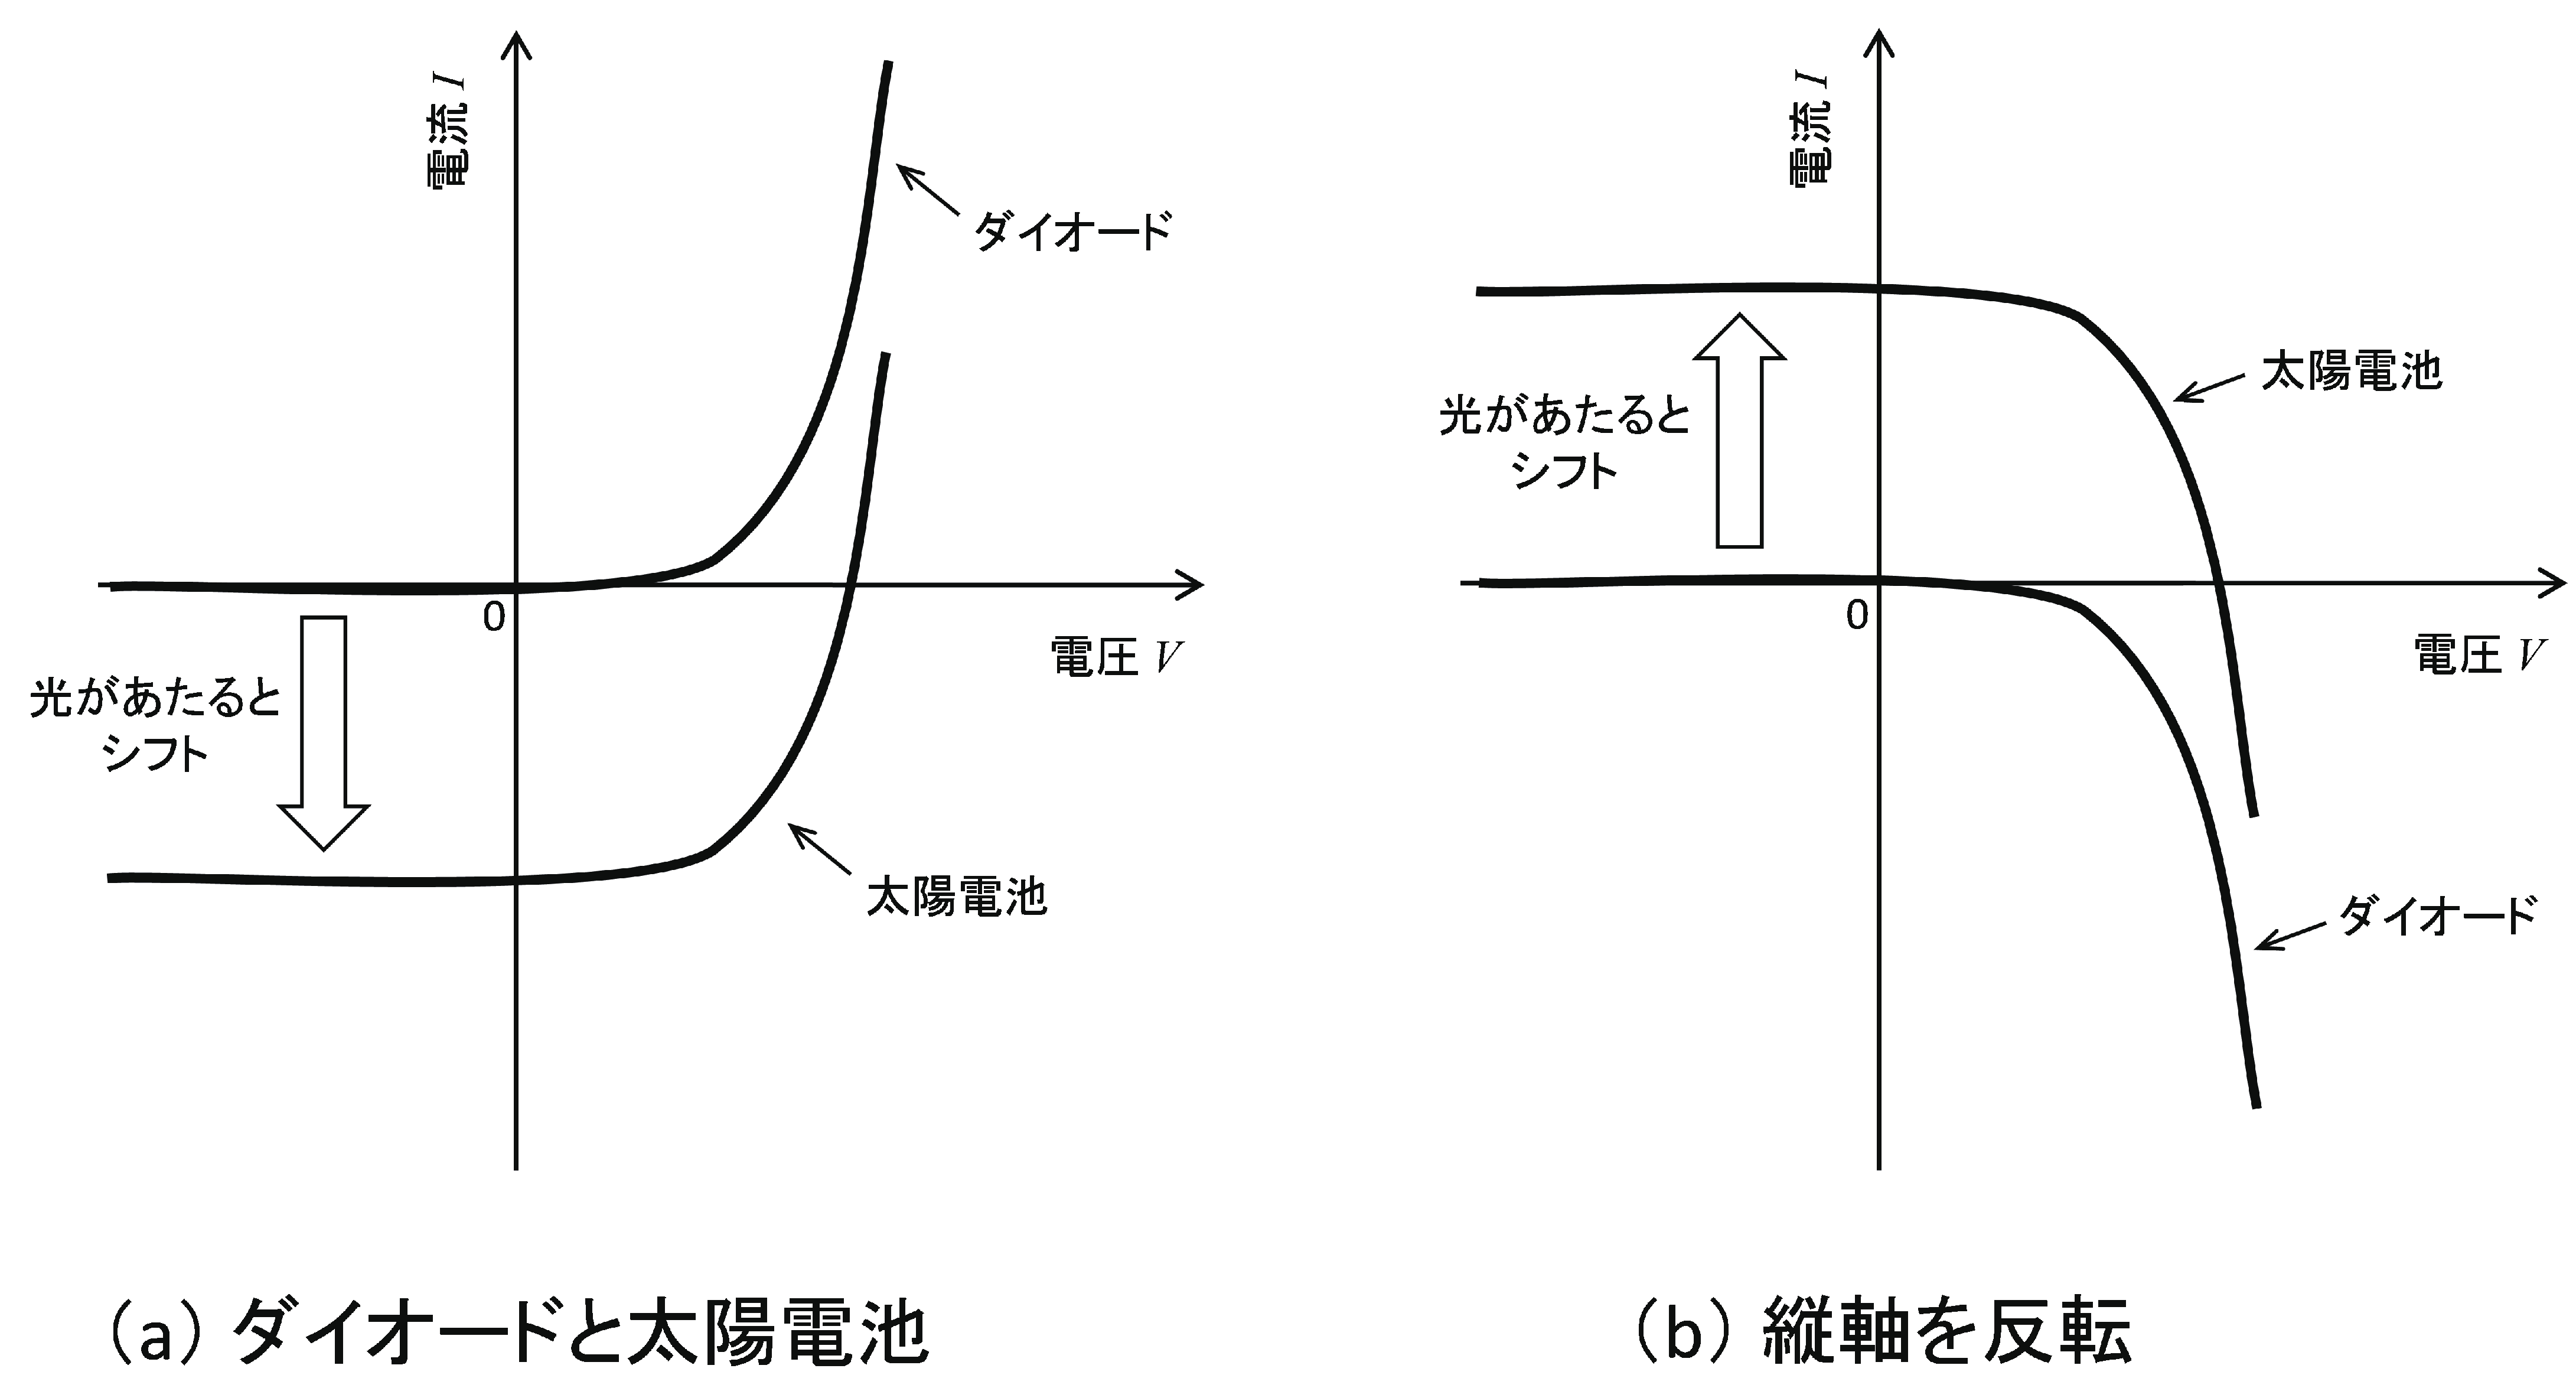
\includegraphics[width=8.5cm]{./pdfs/fig5.pdf}
	\caption{ダイオードと太陽電池の電流--電圧特性}\
	\label{fig:fig5}
\end{figure}
\begin{figure}[htb]
	\centering
	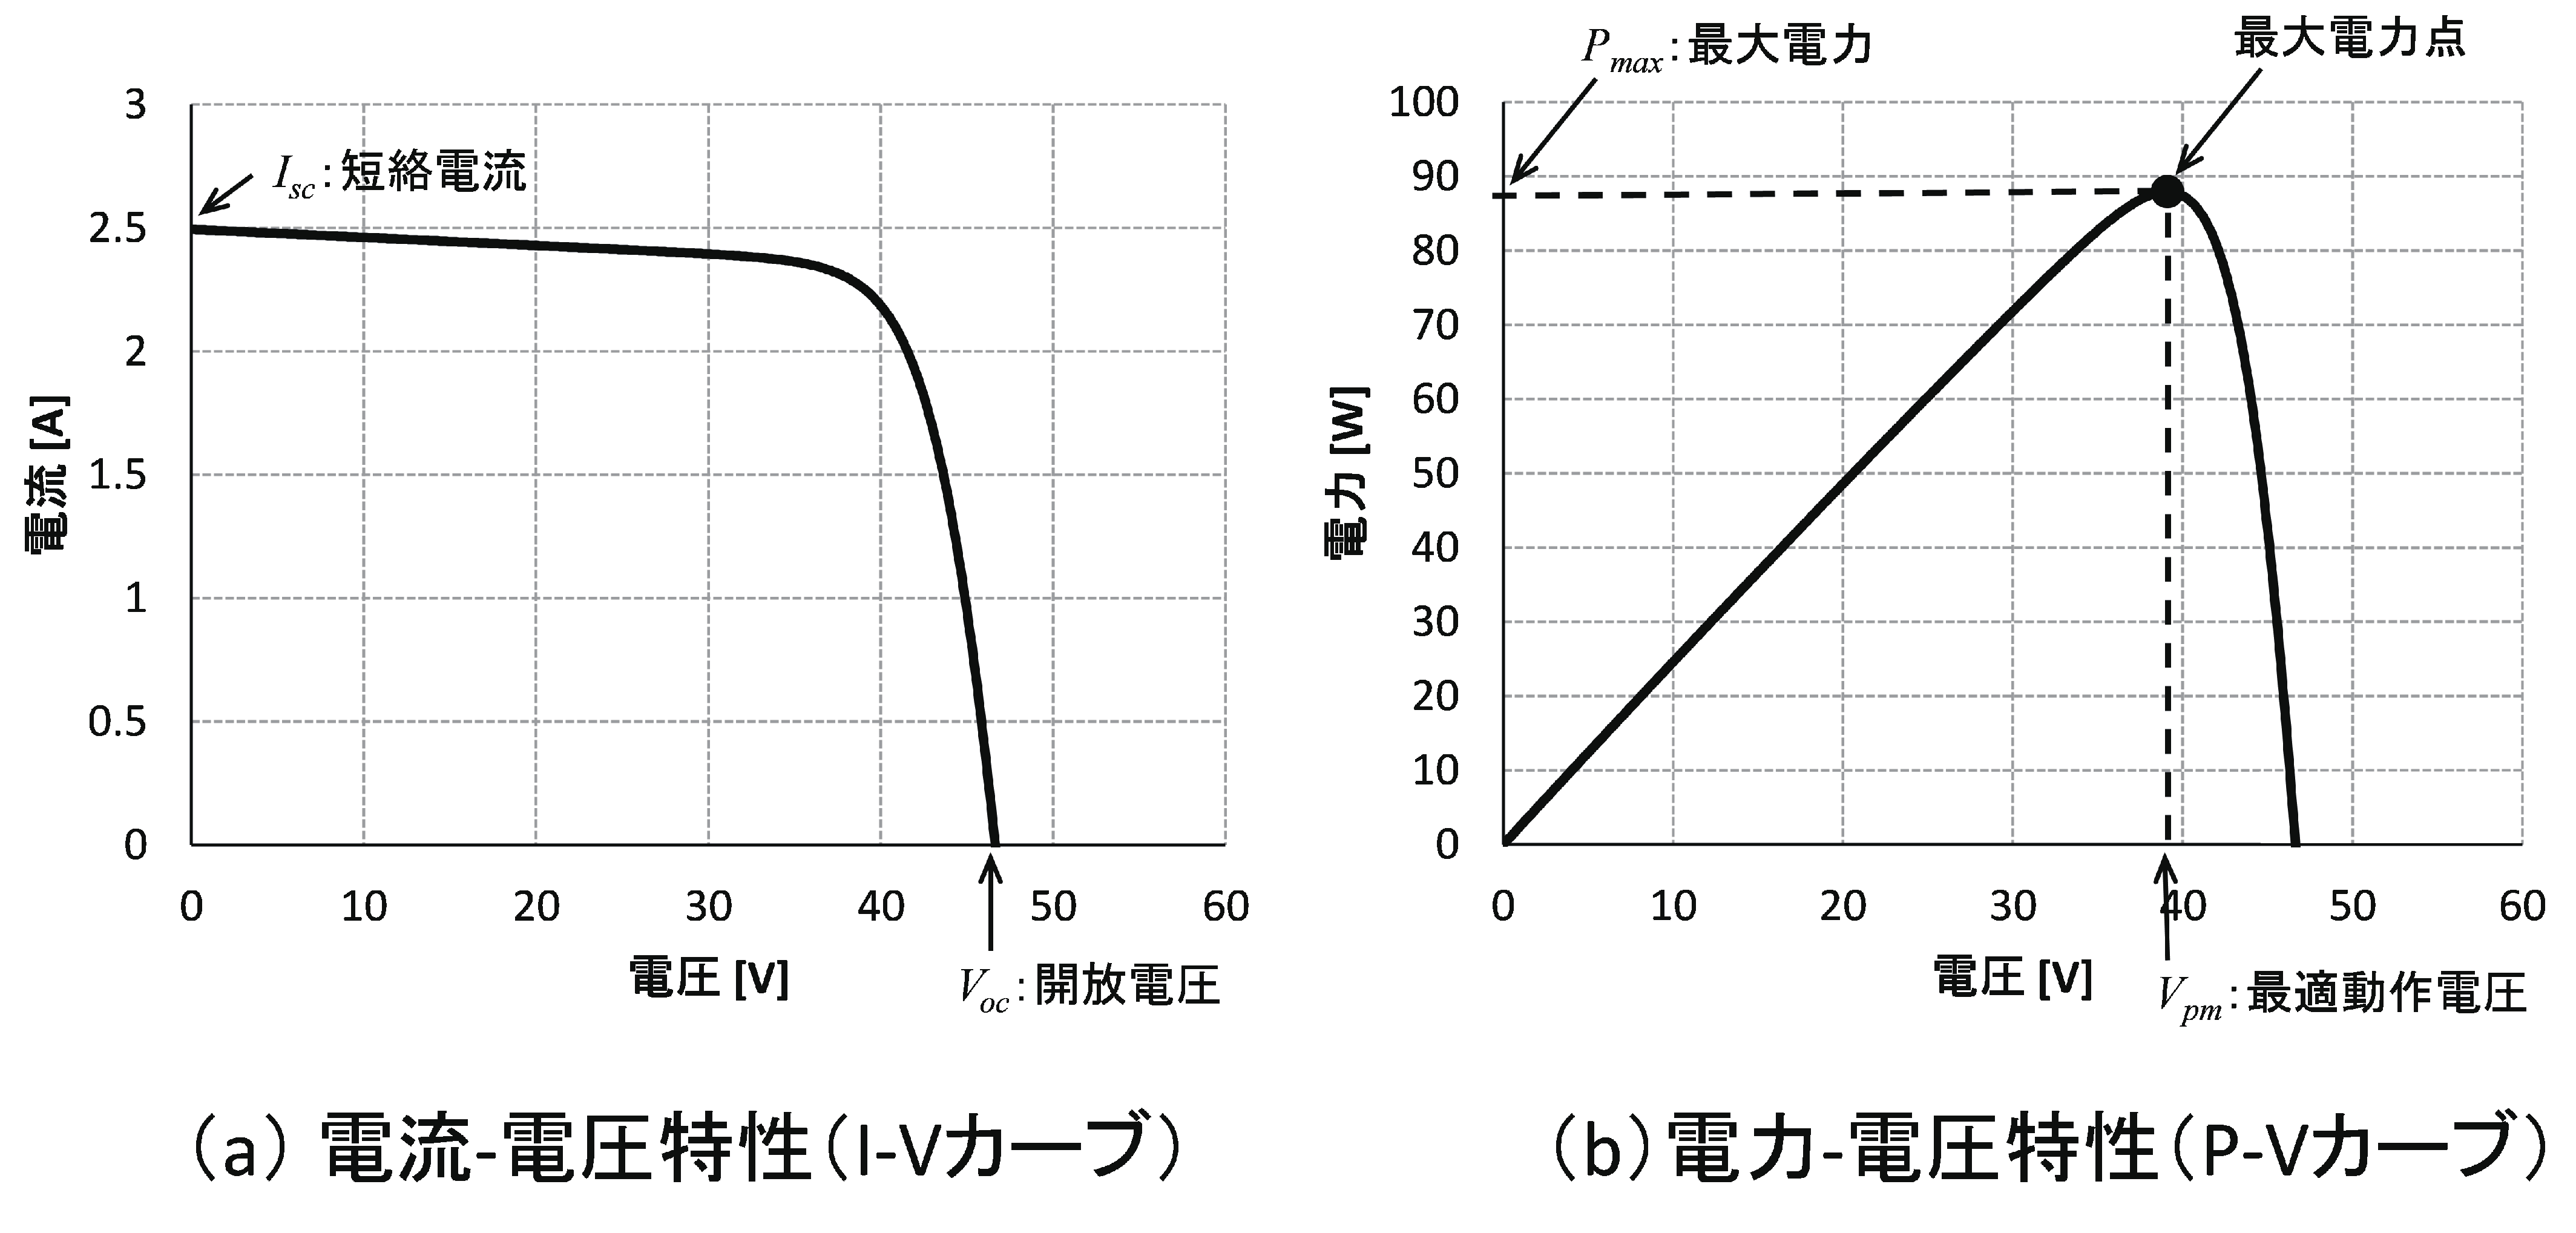
\includegraphics[width=10.3cm]{./pdfs/fig6.pdf}
	\caption{太陽電池の発電特性(左:I--Vカーブ,右:P--Vカーブ)}
	\label{fig:fig6}
\end{figure}%
\clearpage
